
\documentclass{article}
\usepackage{graphicx}
\usepackage[paperheight=40in,paperwidth=30in]{geometry}
 \geometry{
%  a4paper,
 total={170mm,257mm},
 left=3mm,
 right=3mm,
 top=3mm,
 bottom=3mm,
 }
\usepackage{rotating}
\usepackage{adjustbox}

\begin{document}

    \fontsize{32}{32}\selectfont % Sets font size to 14pt with 16pt line spacing
    \vspace*{12mm}
    \centerline{\textbf{aerial}}
    \vspace*{12mm}
    \normalsize % Resets to the base font size
    \def\arraystretch{0.2} % Adjust row spacing if needed
    \fontsize{12}{12}

    \begin{tabular}{ @{}c@{\hspace{0pt}}ccccccc }
        \multicolumn{1}{c}{} &
            \textbf{Thresholds} &
            \textbf{PSNR-vs-Level} &
            \textbf{Level 2} &
            \textbf{Level 4} &
            \textbf{Level 6} &
            \textbf{Level 8} &
            \textbf{Level 10} \\
        \vspace*{10mm}
        \adjustbox{valign=c}{\rotatebox[origin=c]{90}{\textbf{ aerial mean }}} &
            \adjustbox{valign=c}{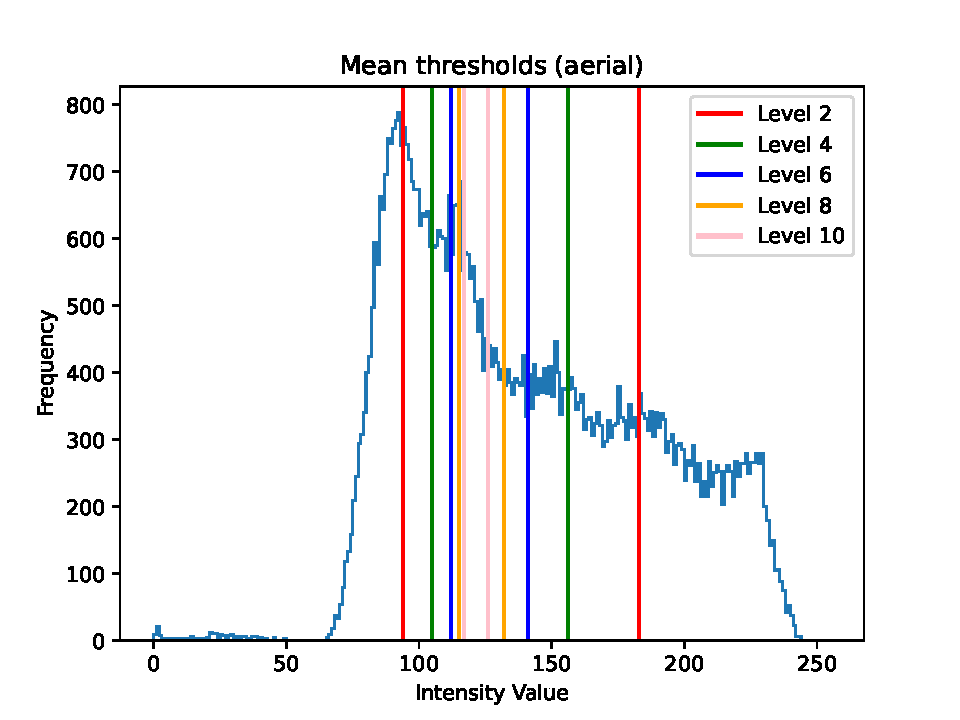
\includegraphics[width=0.13\columnwidth]{../test_results/aerial_mean.pdf}}&
            \adjustbox{valign=c}{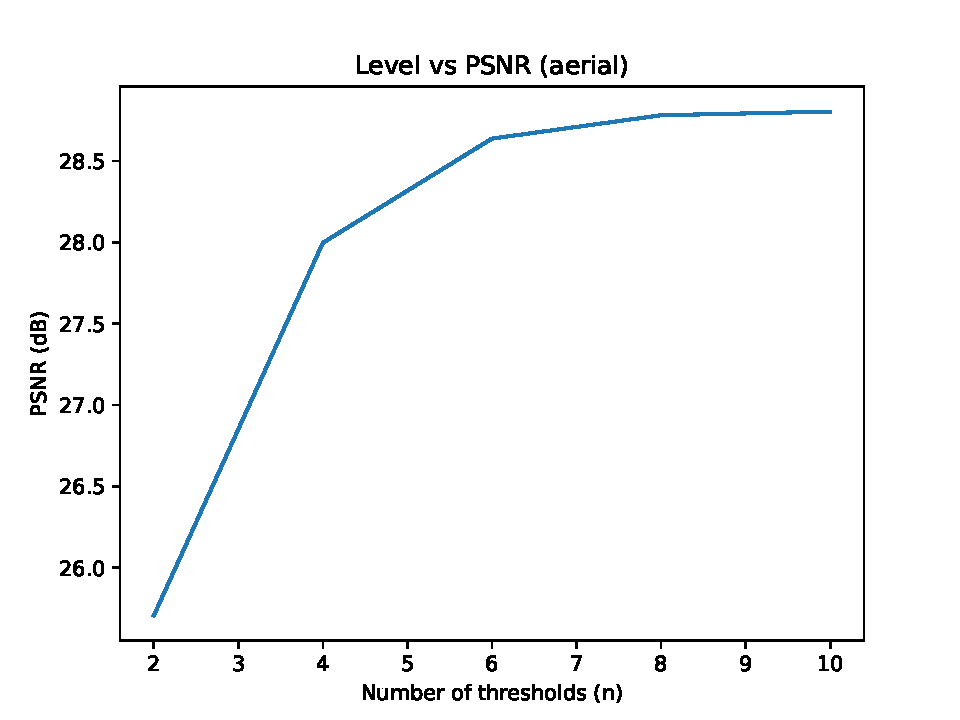
\includegraphics[width=0.13\columnwidth]{../test_results/aerial_mean_psnr.pdf}}&
            \adjustbox{valign=c}{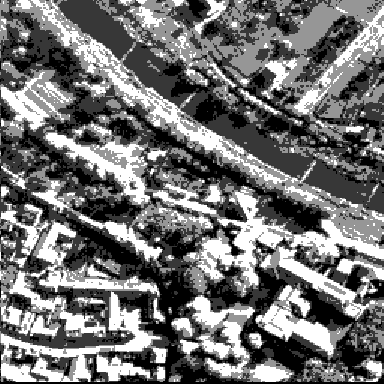
\includegraphics[width=0.13\columnwidth]{../test_results/aerial_2_mean_img.pdf}}&
            \adjustbox{valign=c}{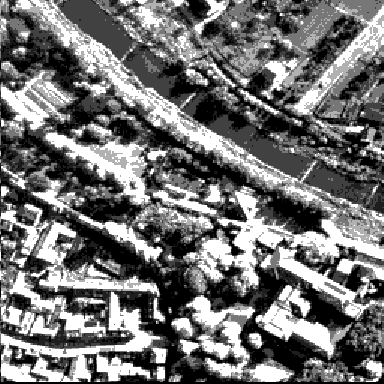
\includegraphics[width=0.13\columnwidth]{../test_results/aerial_4_mean_img.pdf}}&
            \adjustbox{valign=c}{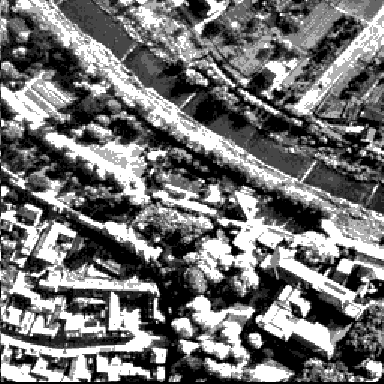
\includegraphics[width=0.13\columnwidth]{../test_results/aerial_6_mean_img.pdf}}&
            \adjustbox{valign=c}{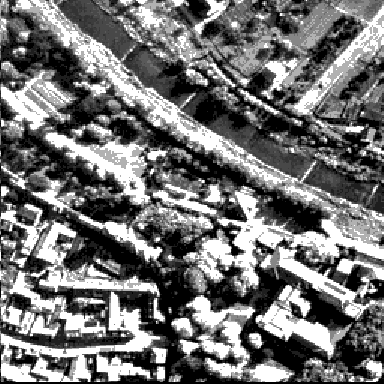
\includegraphics[width=0.13\columnwidth]{../test_results/aerial_8_mean_img.pdf}}&
            \adjustbox{valign=c}{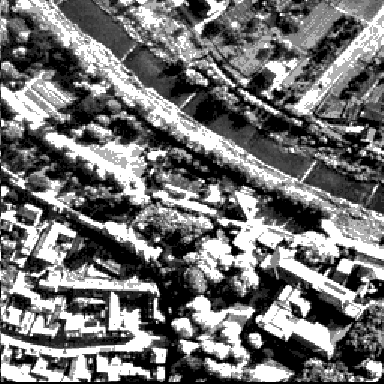
\includegraphics[width=0.13\columnwidth]{../test_results/aerial_10_mean_img.pdf}}\\
        \vspace*{6mm}
        \adjustbox{valign=c}{\rotatebox[origin=c]{90}{\textbf{ aerial mode }}} &
            \adjustbox{valign=c}{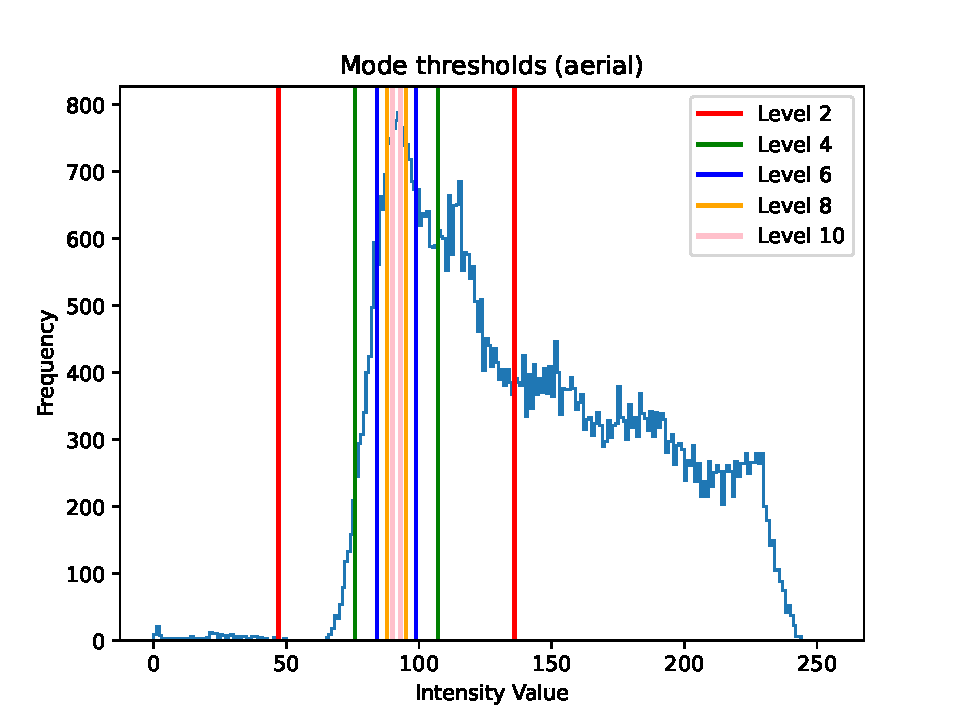
\includegraphics[width=0.13\columnwidth]{../test_results/aerial_mode.pdf}}&
            \adjustbox{valign=c}{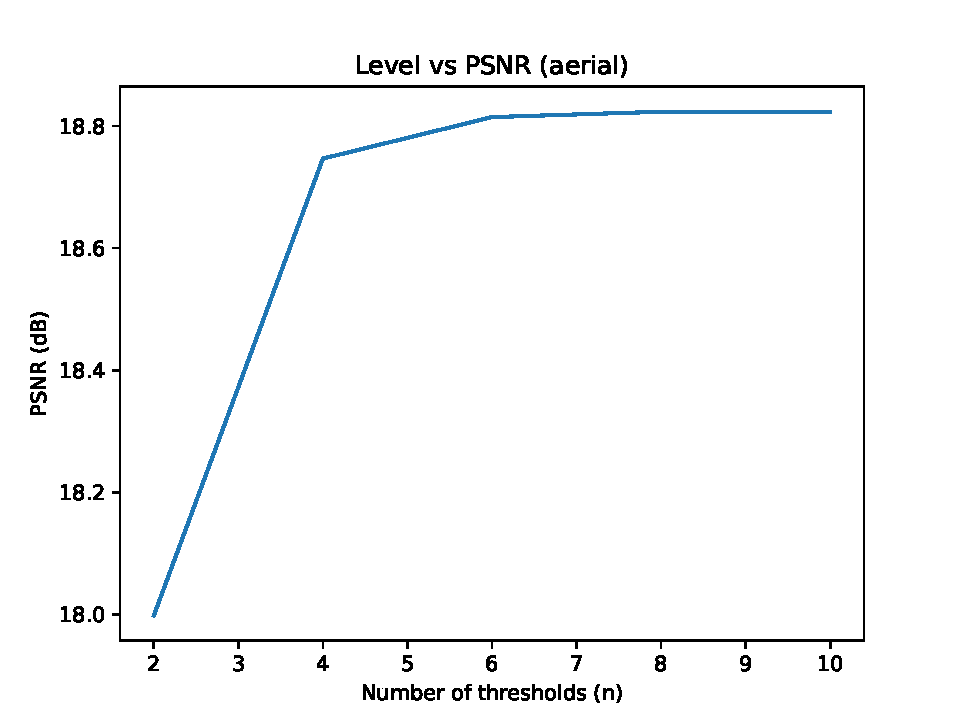
\includegraphics[width=0.13\columnwidth]{../test_results/aerial_mode_psnr.pdf}}&
            \adjustbox{valign=c}{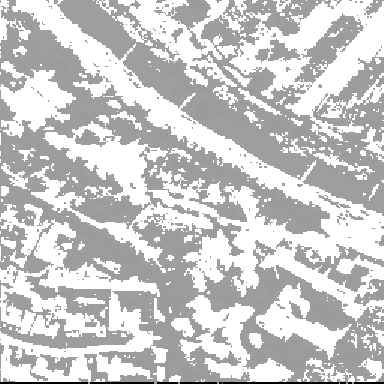
\includegraphics[width=0.13\columnwidth]{../test_results/aerial_2_mode_img.pdf}}&
            \adjustbox{valign=c}{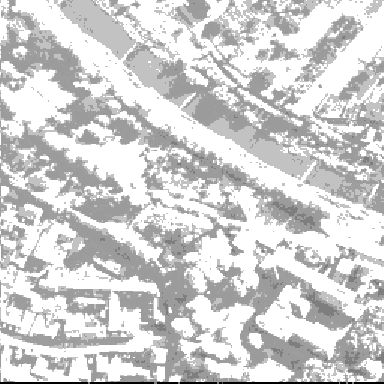
\includegraphics[width=0.13\columnwidth]{../test_results/aerial_4_mode_img.pdf}}&
            \adjustbox{valign=c}{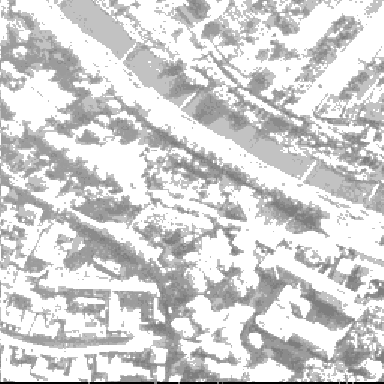
\includegraphics[width=0.13\columnwidth]{../test_results/aerial_6_mode_img.pdf}}&
            \adjustbox{valign=c}{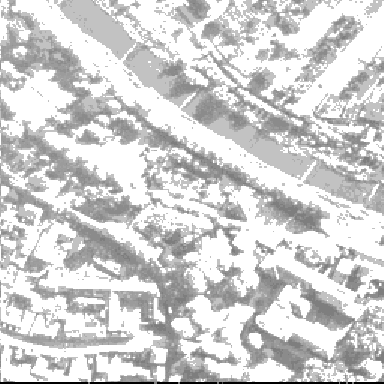
\includegraphics[width=0.13\columnwidth]{../test_results/aerial_8_mode_img.pdf}}&
            \adjustbox{valign=c}{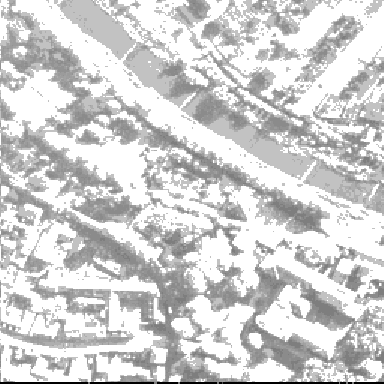
\includegraphics[width=0.13\columnwidth]{../test_results/aerial_10_mode_img.pdf}}\\
    \end{tabular}
    \bigskip
                
        
    \fontsize{32}{32}\selectfont % Sets font size to 14pt with 16pt line spacing
    \vspace*{12mm}
    \centerline{\textbf{baboon}}
    \vspace*{12mm}
    \normalsize % Resets to the base font size
    \def\arraystretch{0.2} % Adjust row spacing if needed
    \fontsize{12}{12}

    \begin{tabular}{ @{}c@{\hspace{0pt}}ccccccc }
        \multicolumn{1}{c}{} &
            \textbf{Thresholds} &
            \textbf{PSNR-vs-Level} &
            \textbf{Level 2} &
            \textbf{Level 4} &
            \textbf{Level 6} &
            \textbf{Level 8} &
            \textbf{Level 10} \\
        \vspace*{10mm}
        \adjustbox{valign=c}{\rotatebox[origin=c]{90}{\textbf{ baboon mean }}} &
            \adjustbox{valign=c}{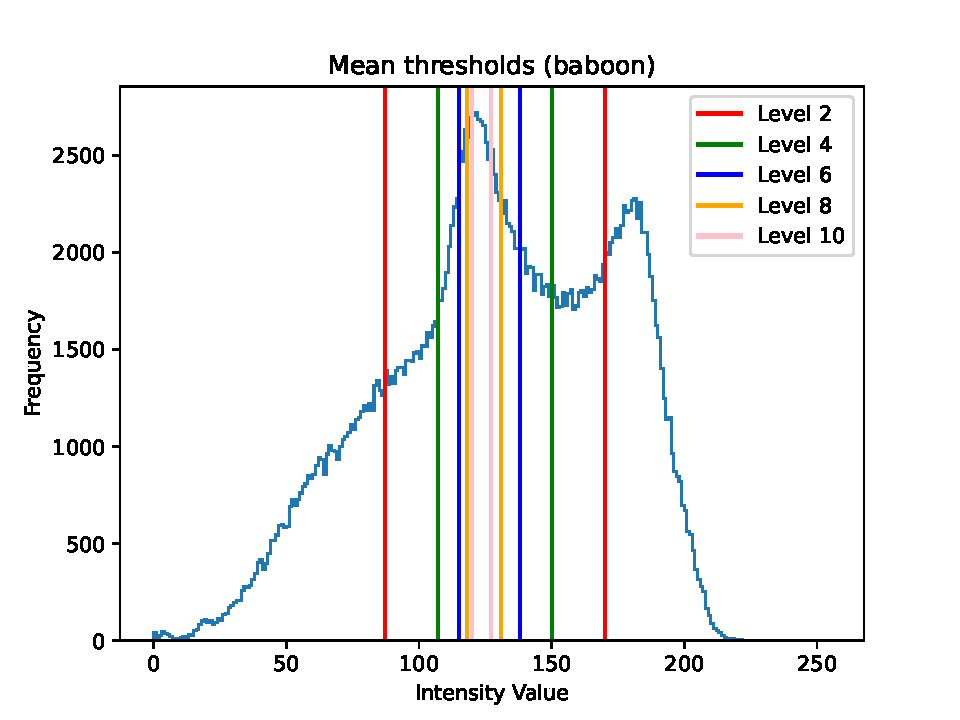
\includegraphics[width=0.13\columnwidth]{../test_results/baboon_mean.pdf}}&
            \adjustbox{valign=c}{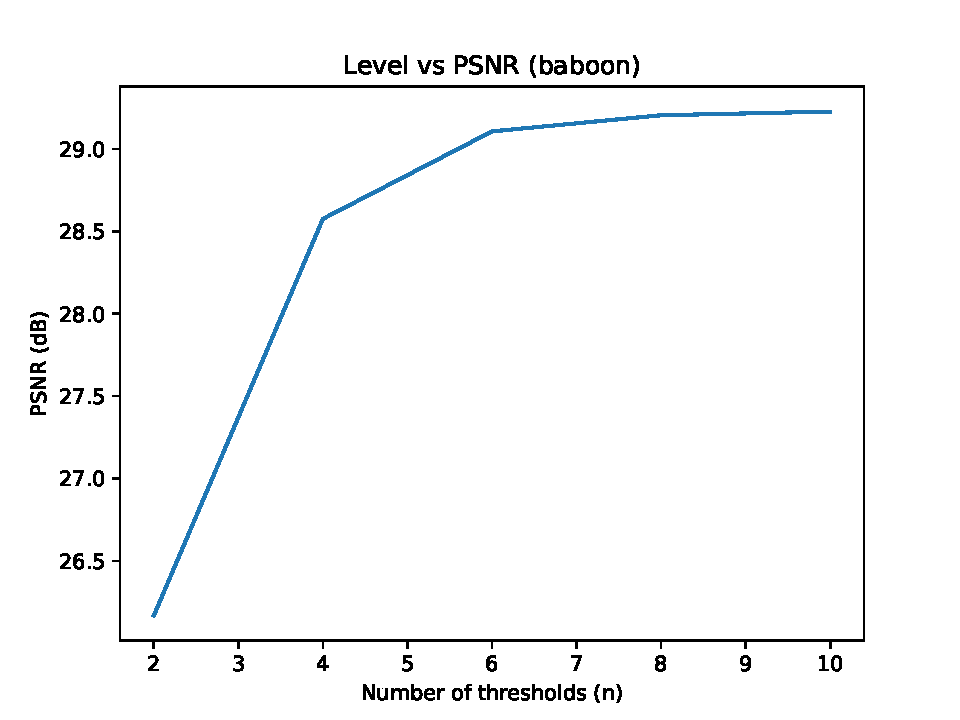
\includegraphics[width=0.13\columnwidth]{../test_results/baboon_mean_psnr.pdf}}&
            \adjustbox{valign=c}{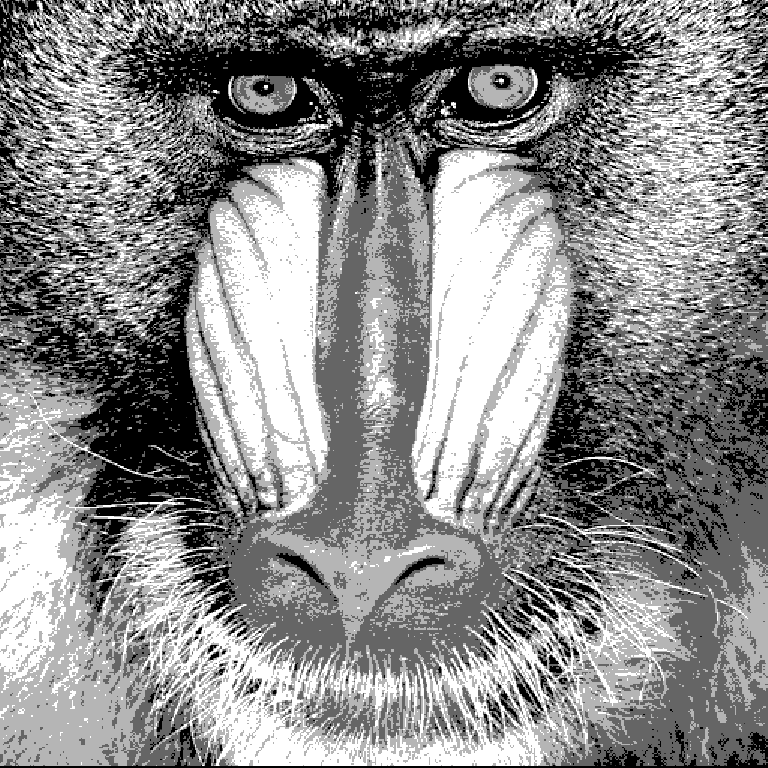
\includegraphics[width=0.13\columnwidth]{../test_results/baboon_2_mean_img.pdf}}&
            \adjustbox{valign=c}{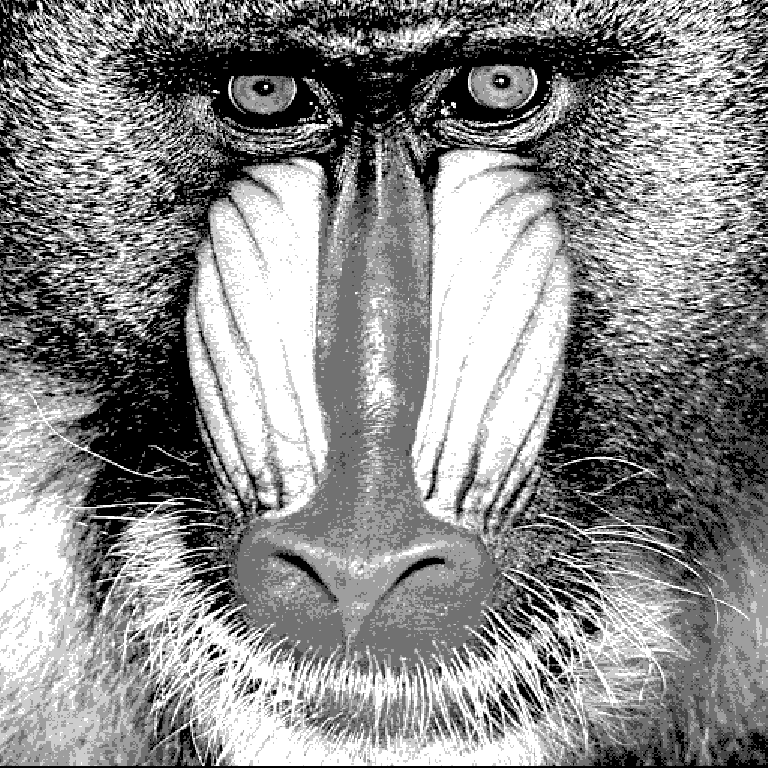
\includegraphics[width=0.13\columnwidth]{../test_results/baboon_4_mean_img.pdf}}&
            \adjustbox{valign=c}{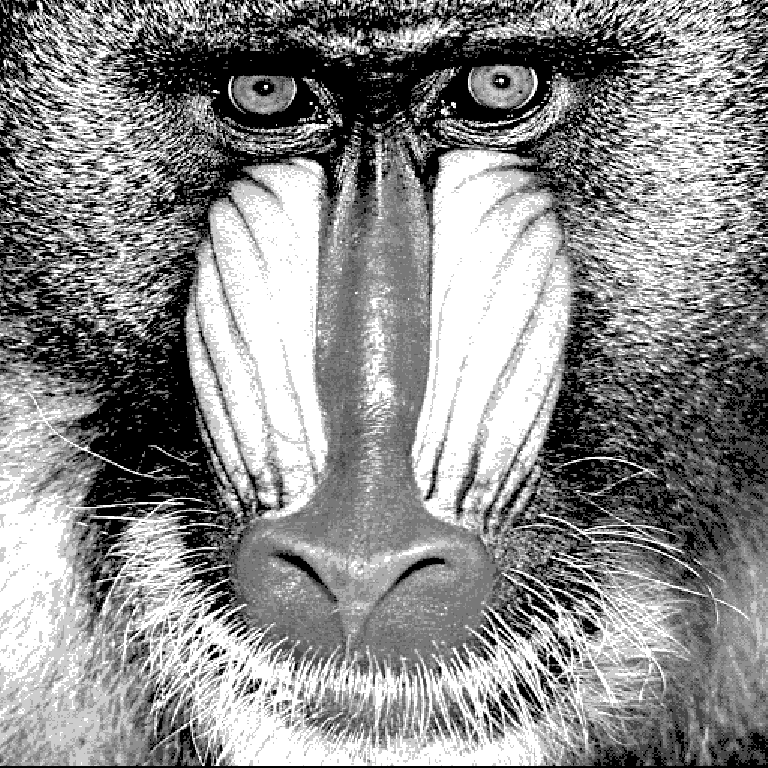
\includegraphics[width=0.13\columnwidth]{../test_results/baboon_6_mean_img.pdf}}&
            \adjustbox{valign=c}{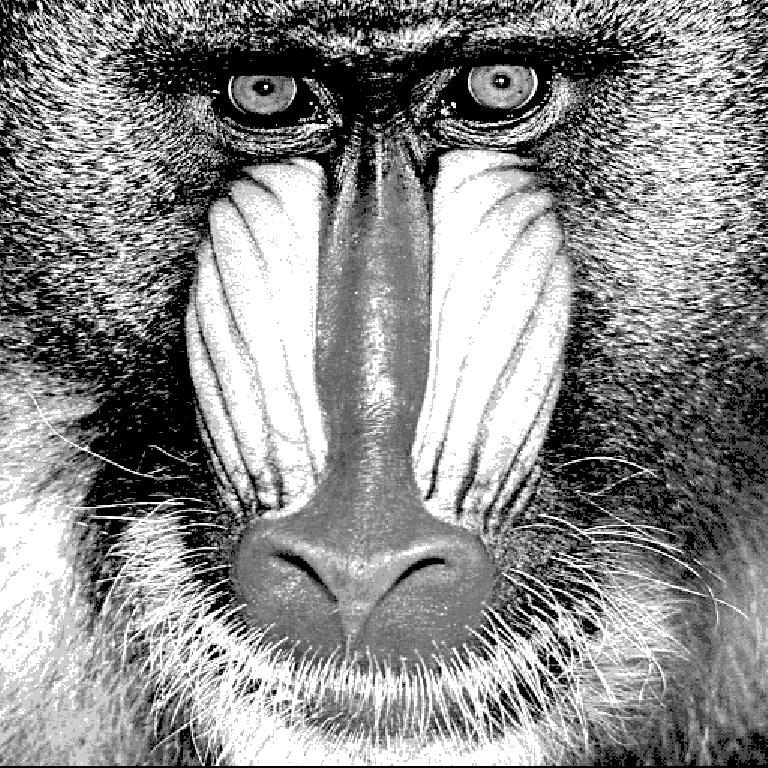
\includegraphics[width=0.13\columnwidth]{../test_results/baboon_8_mean_img.pdf}}&
            \adjustbox{valign=c}{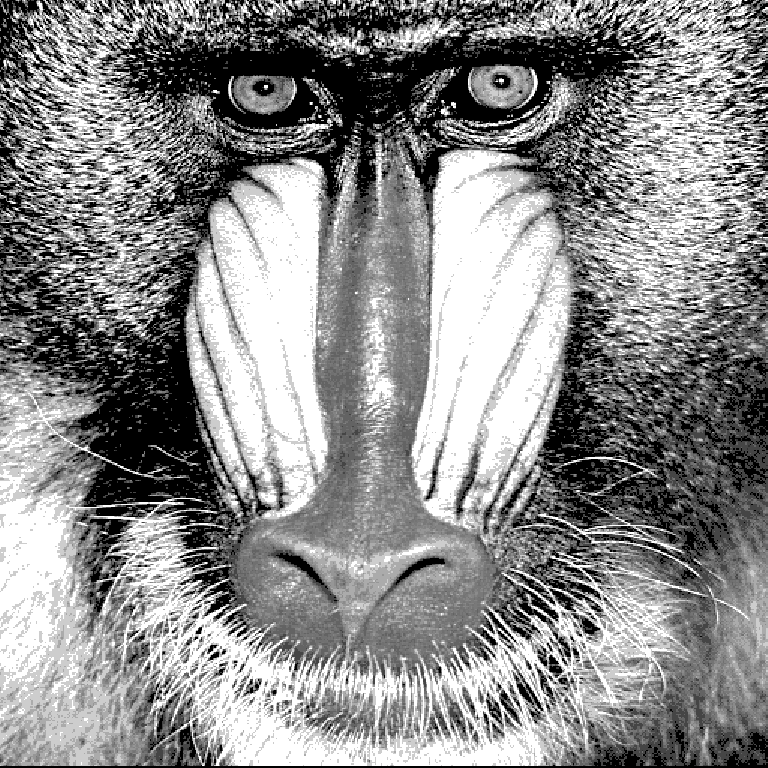
\includegraphics[width=0.13\columnwidth]{../test_results/baboon_10_mean_img.pdf}}\\
        \vspace*{6mm}
        \adjustbox{valign=c}{\rotatebox[origin=c]{90}{\textbf{ baboon mode }}} &
            \adjustbox{valign=c}{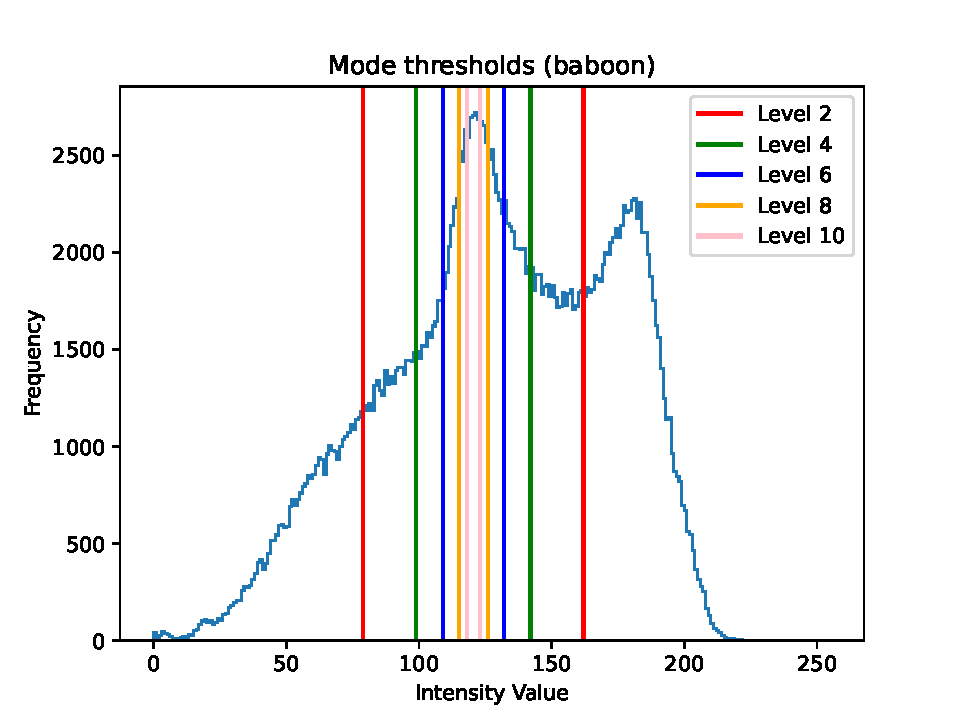
\includegraphics[width=0.13\columnwidth]{../test_results/baboon_mode.pdf}}&
            \adjustbox{valign=c}{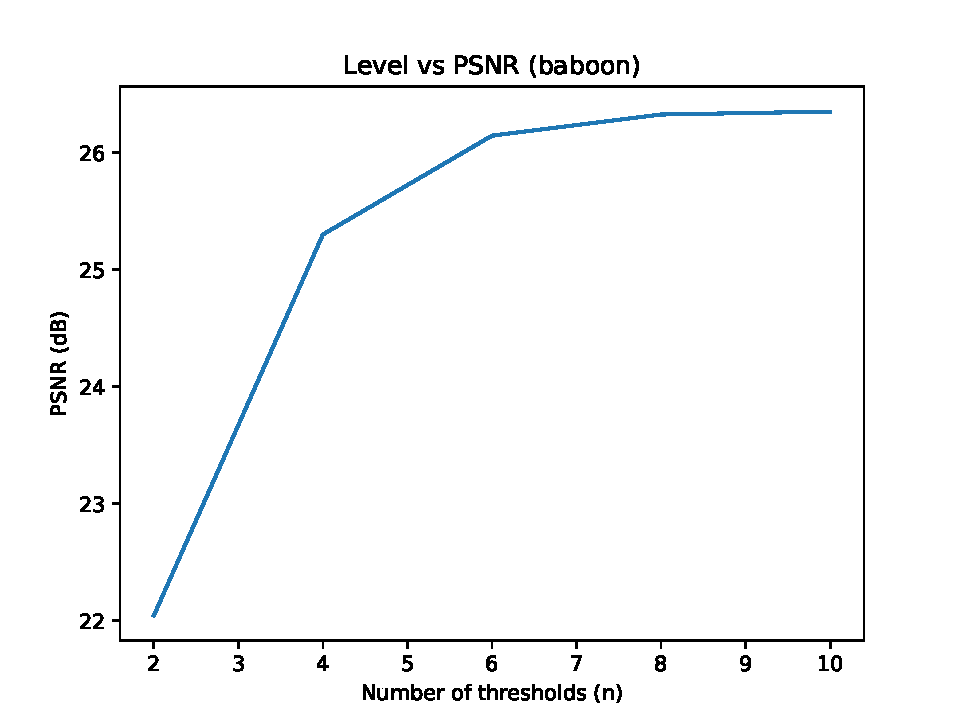
\includegraphics[width=0.13\columnwidth]{../test_results/baboon_mode_psnr.pdf}}&
            \adjustbox{valign=c}{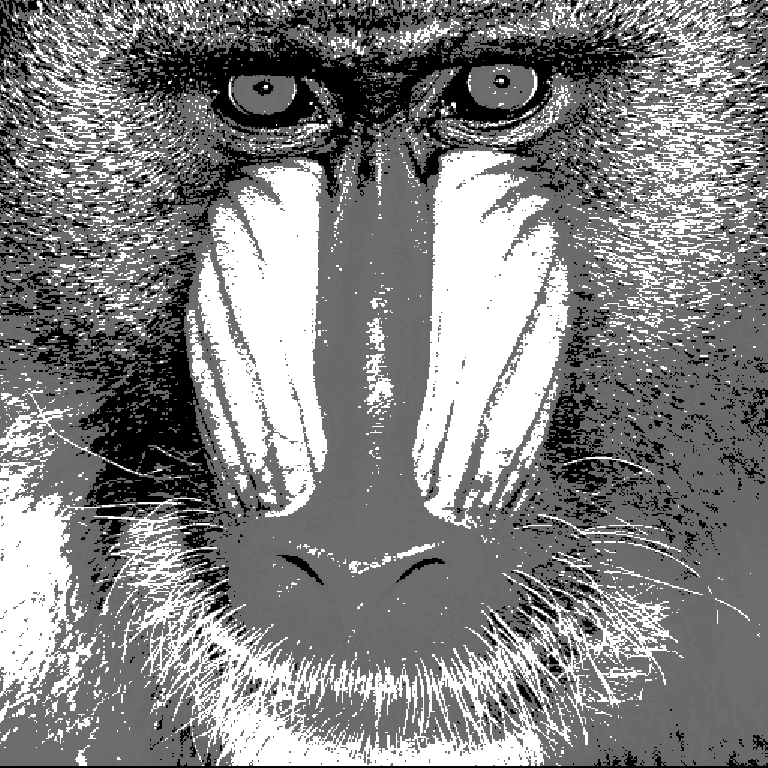
\includegraphics[width=0.13\columnwidth]{../test_results/baboon_2_mode_img.pdf}}&
            \adjustbox{valign=c}{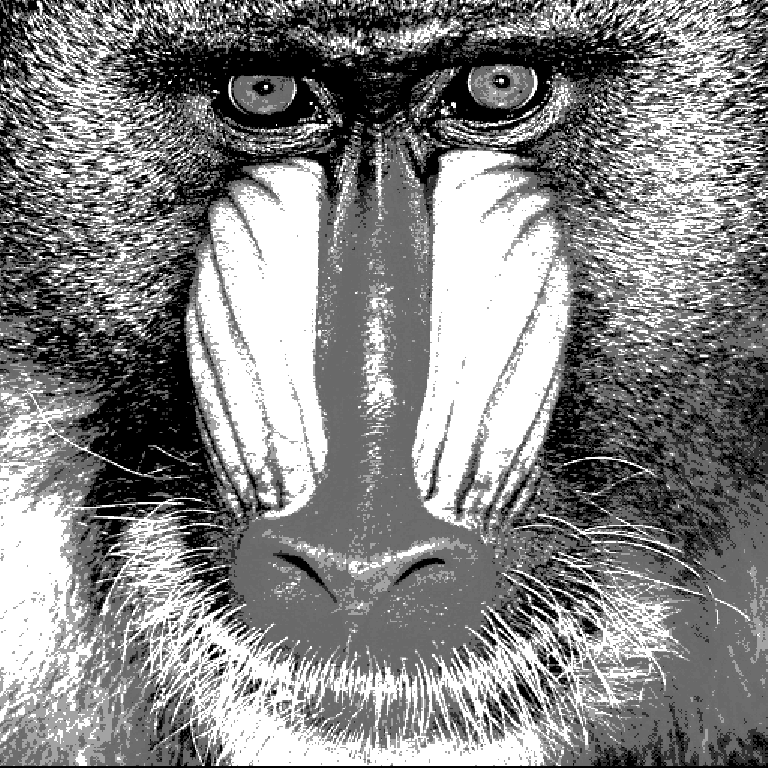
\includegraphics[width=0.13\columnwidth]{../test_results/baboon_4_mode_img.pdf}}&
            \adjustbox{valign=c}{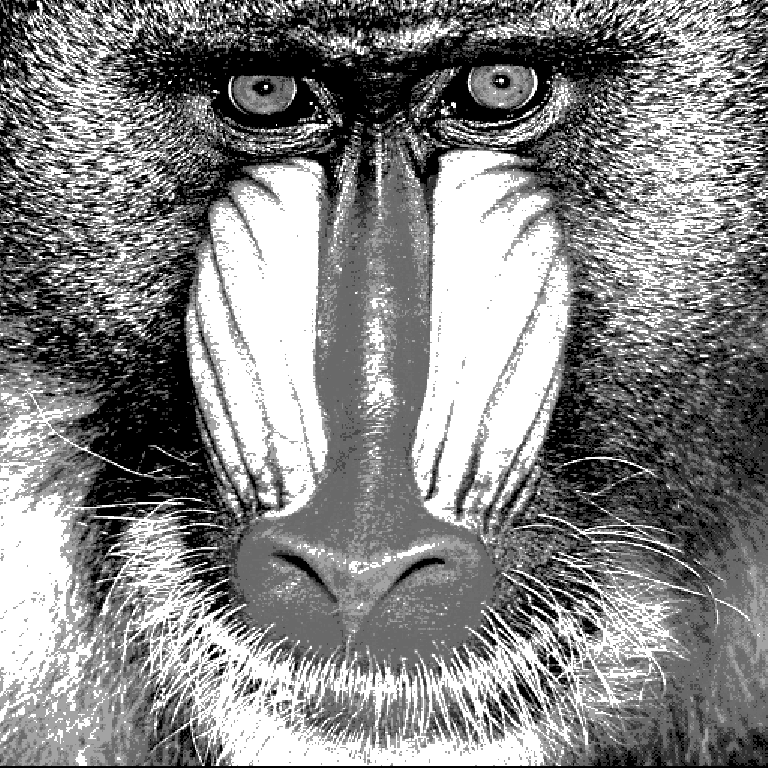
\includegraphics[width=0.13\columnwidth]{../test_results/baboon_6_mode_img.pdf}}&
            \adjustbox{valign=c}{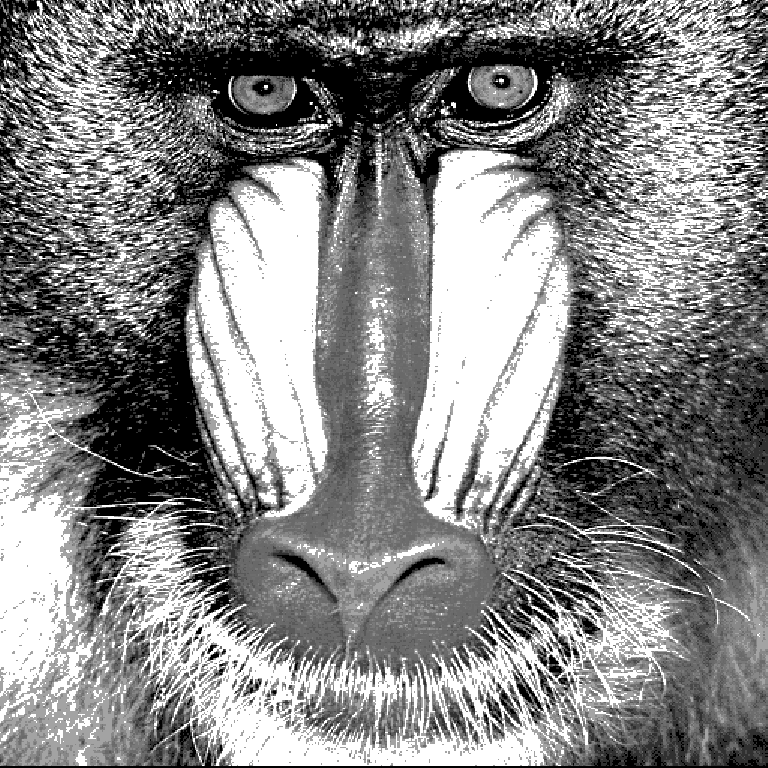
\includegraphics[width=0.13\columnwidth]{../test_results/baboon_8_mode_img.pdf}}&
            \adjustbox{valign=c}{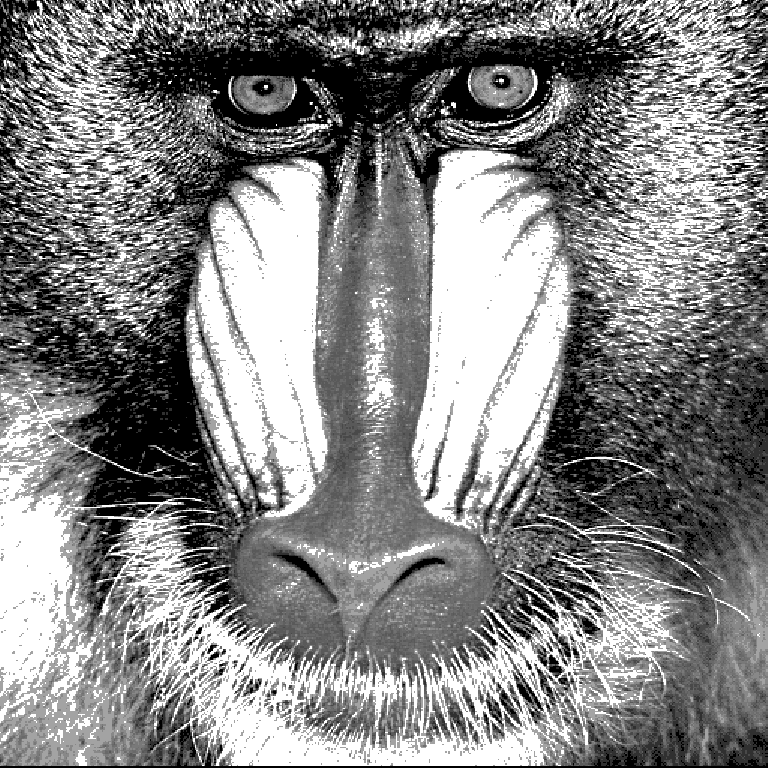
\includegraphics[width=0.13\columnwidth]{../test_results/baboon_10_mode_img.pdf}}\\
    \end{tabular}
    \bigskip
                
        
    \fontsize{32}{32}\selectfont % Sets font size to 14pt with 16pt line spacing
    \vspace*{12mm}
    \centerline{\textbf{boat}}
    \vspace*{12mm}
    \normalsize % Resets to the base font size
    \def\arraystretch{0.2} % Adjust row spacing if needed
    \fontsize{12}{12}

    \begin{tabular}{ @{}c@{\hspace{0pt}}ccccccc }
        \multicolumn{1}{c}{} &
            \textbf{Thresholds} &
            \textbf{PSNR-vs-Level} &
            \textbf{Level 2} &
            \textbf{Level 4} &
            \textbf{Level 6} &
            \textbf{Level 8} &
            \textbf{Level 10} \\
        \vspace*{10mm}
        \adjustbox{valign=c}{\rotatebox[origin=c]{90}{\textbf{ boat mean }}} &
            \adjustbox{valign=c}{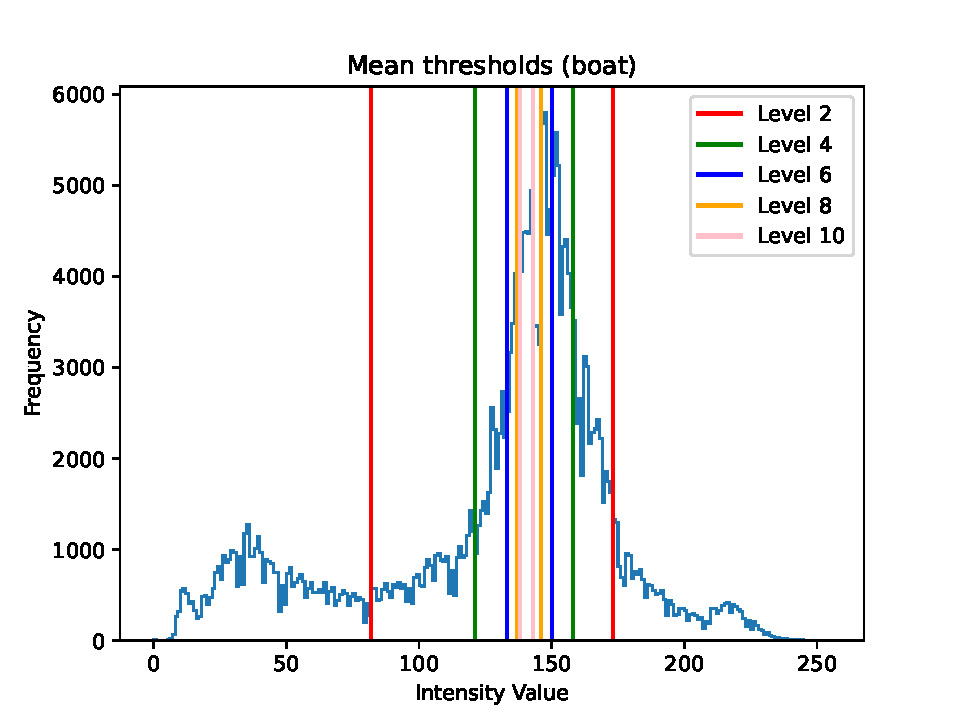
\includegraphics[width=0.13\columnwidth]{../test_results/boat_mean.pdf}}&
            \adjustbox{valign=c}{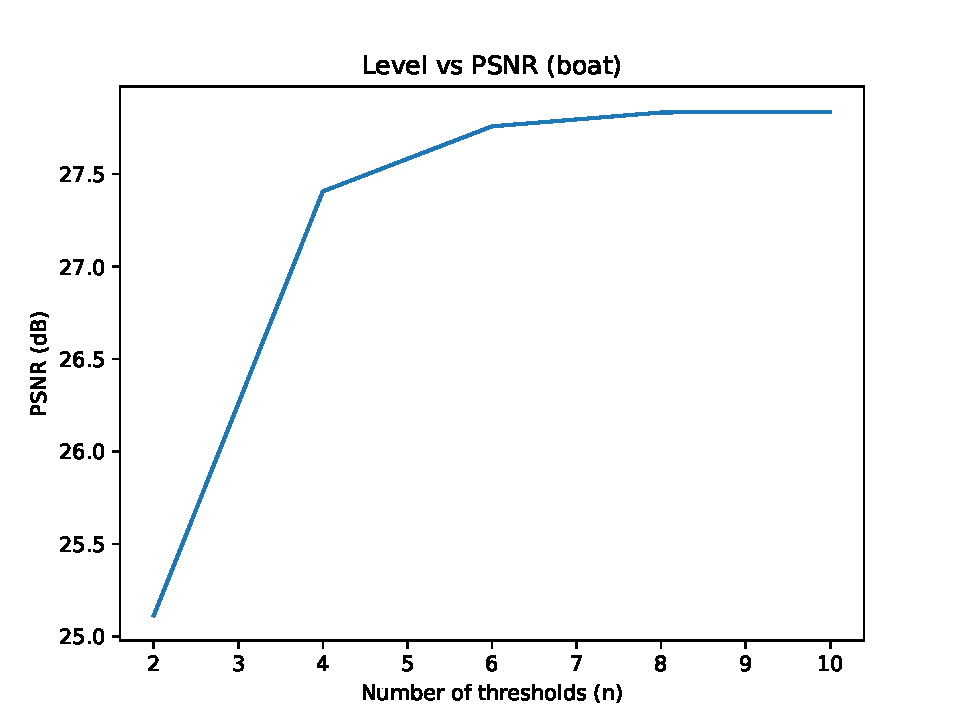
\includegraphics[width=0.13\columnwidth]{../test_results/boat_mean_psnr.pdf}}&
            \adjustbox{valign=c}{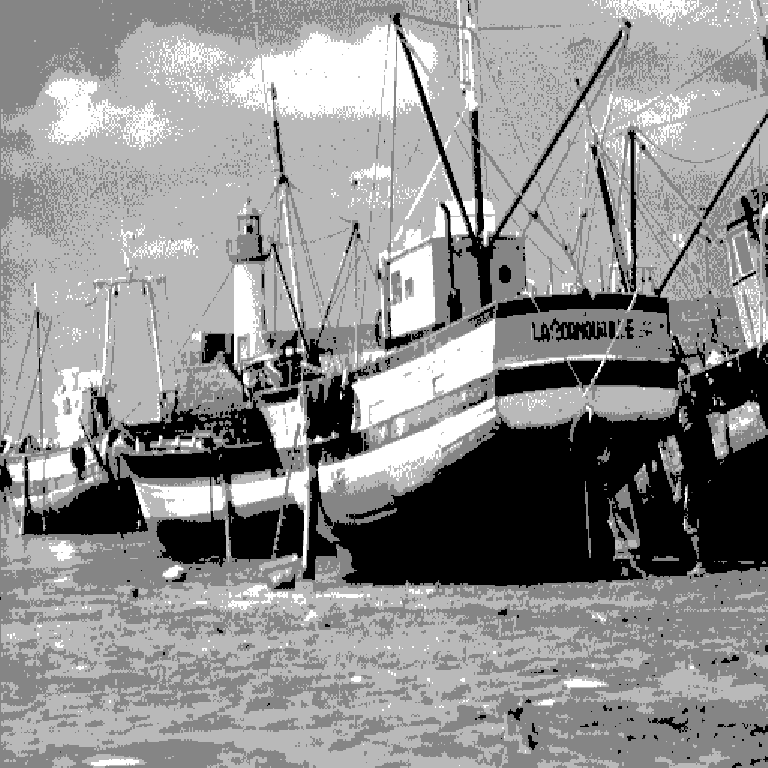
\includegraphics[width=0.13\columnwidth]{../test_results/boat_2_mean_img.pdf}}&
            \adjustbox{valign=c}{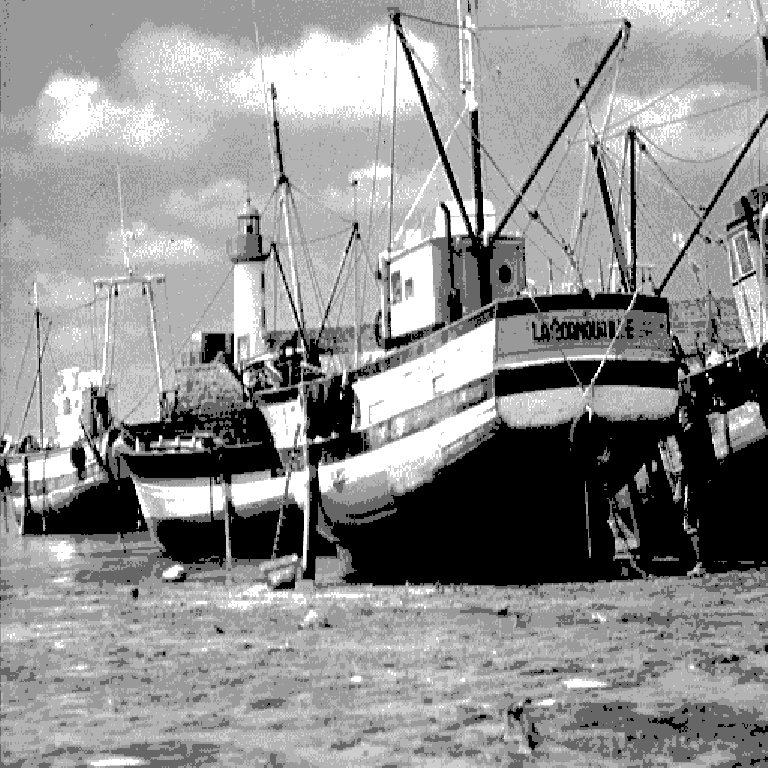
\includegraphics[width=0.13\columnwidth]{../test_results/boat_4_mean_img.pdf}}&
            \adjustbox{valign=c}{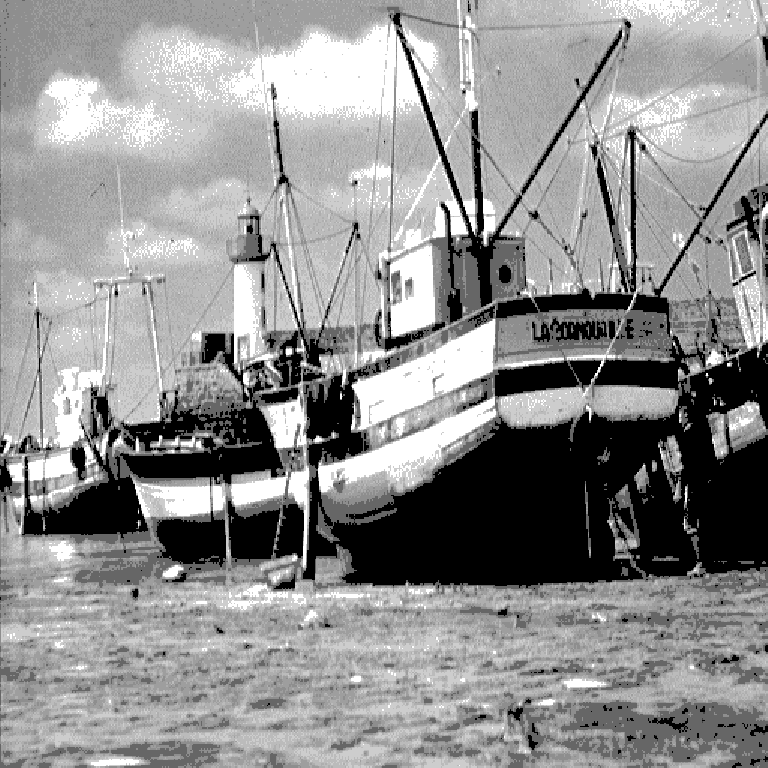
\includegraphics[width=0.13\columnwidth]{../test_results/boat_6_mean_img.pdf}}&
            \adjustbox{valign=c}{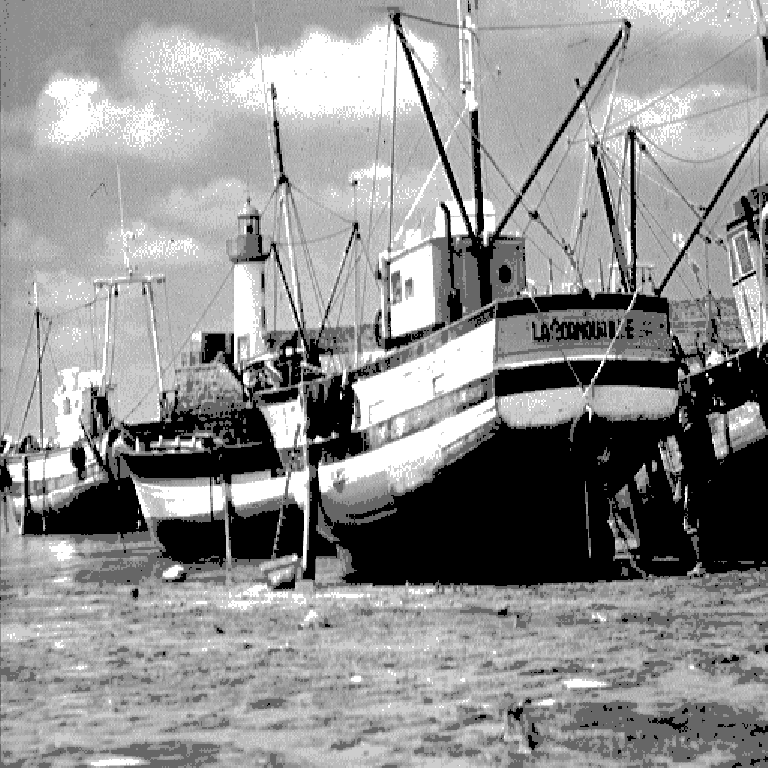
\includegraphics[width=0.13\columnwidth]{../test_results/boat_8_mean_img.pdf}}&
            \adjustbox{valign=c}{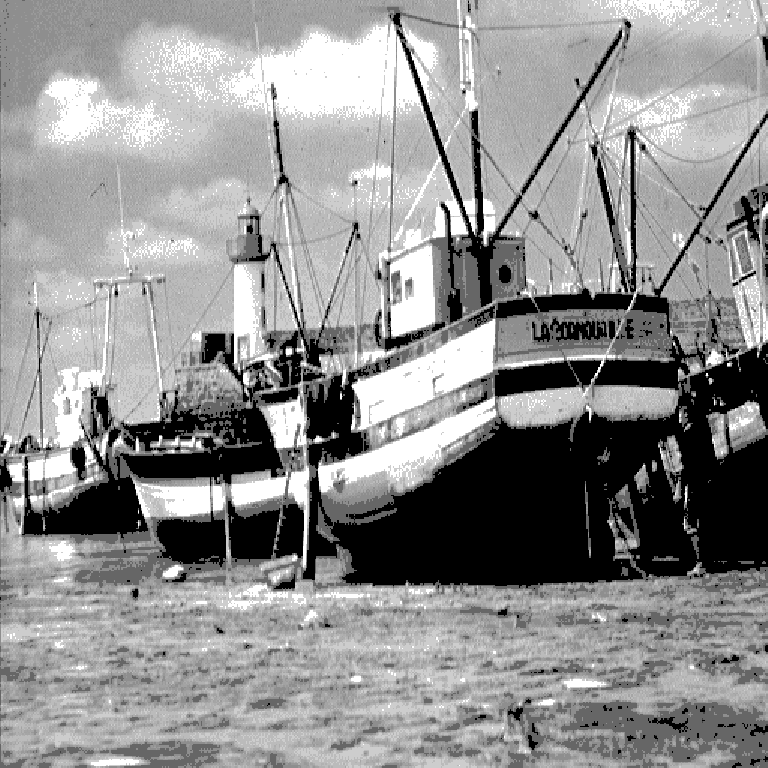
\includegraphics[width=0.13\columnwidth]{../test_results/boat_10_mean_img.pdf}}\\
        \vspace*{6mm}
        \adjustbox{valign=c}{\rotatebox[origin=c]{90}{\textbf{ boat mode }}} &
            \adjustbox{valign=c}{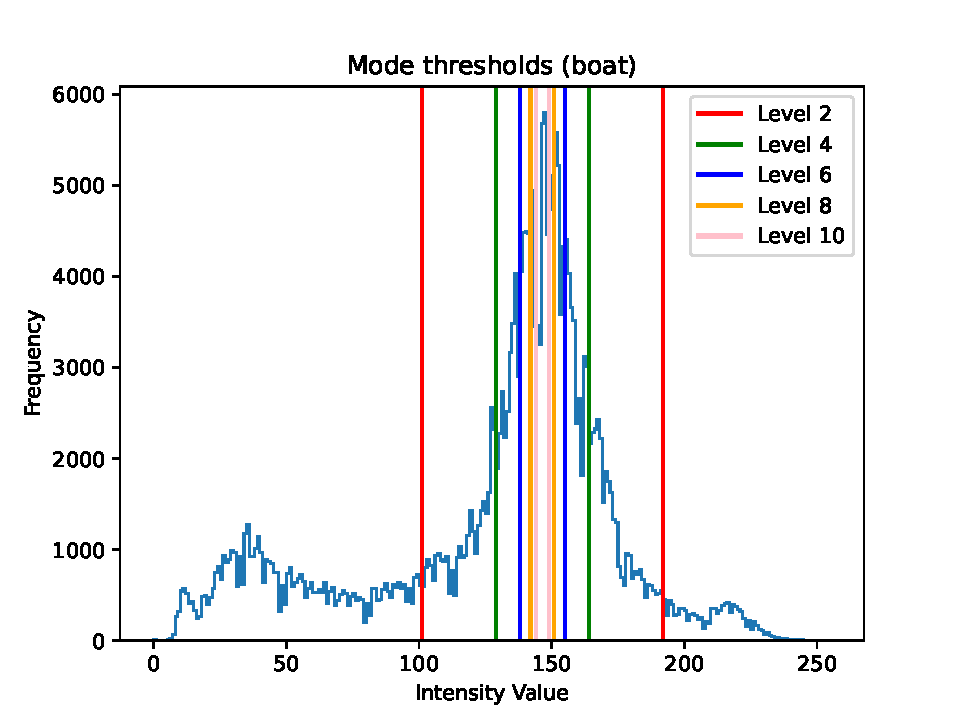
\includegraphics[width=0.13\columnwidth]{../test_results/boat_mode.pdf}}&
            \adjustbox{valign=c}{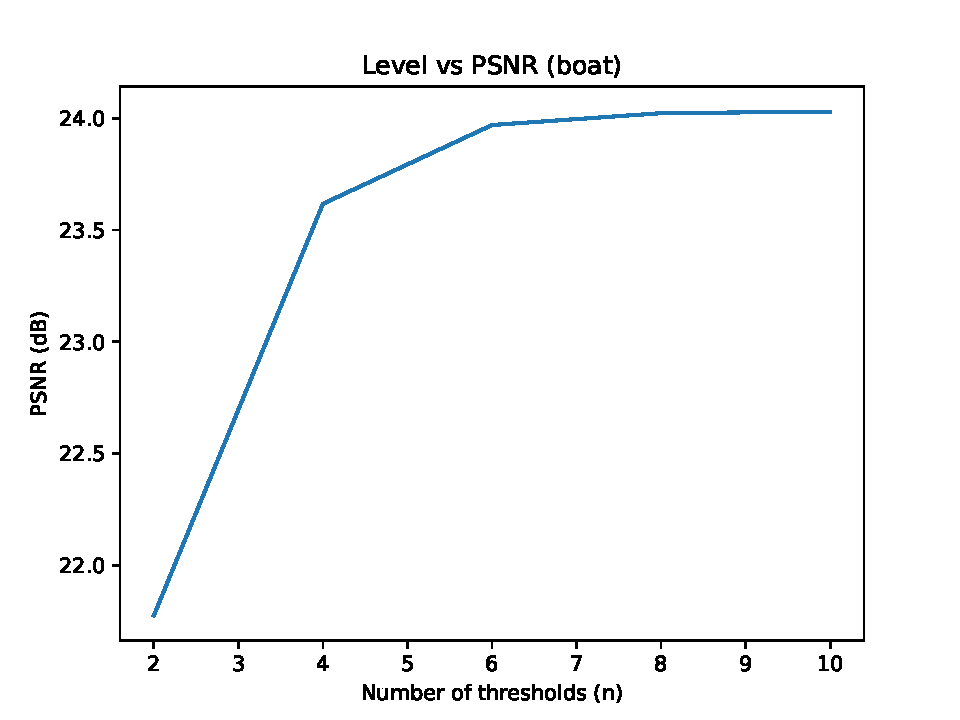
\includegraphics[width=0.13\columnwidth]{../test_results/boat_mode_psnr.pdf}}&
            \adjustbox{valign=c}{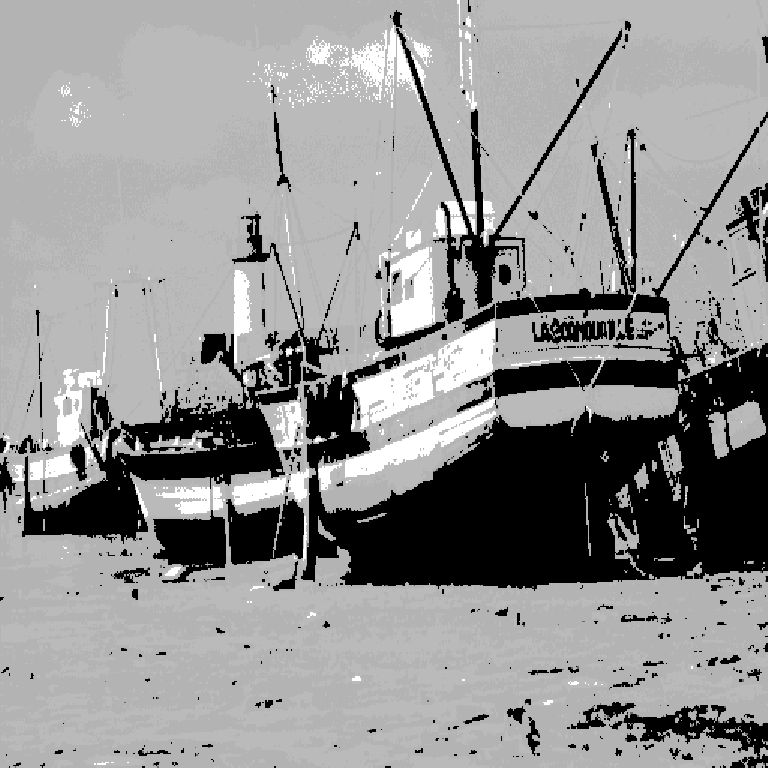
\includegraphics[width=0.13\columnwidth]{../test_results/boat_2_mode_img.pdf}}&
            \adjustbox{valign=c}{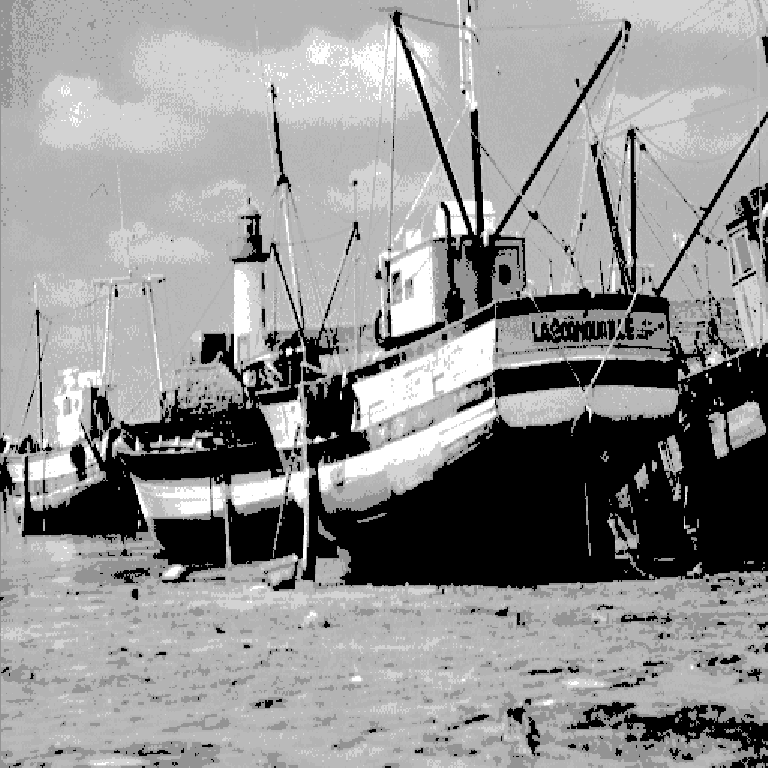
\includegraphics[width=0.13\columnwidth]{../test_results/boat_4_mode_img.pdf}}&
            \adjustbox{valign=c}{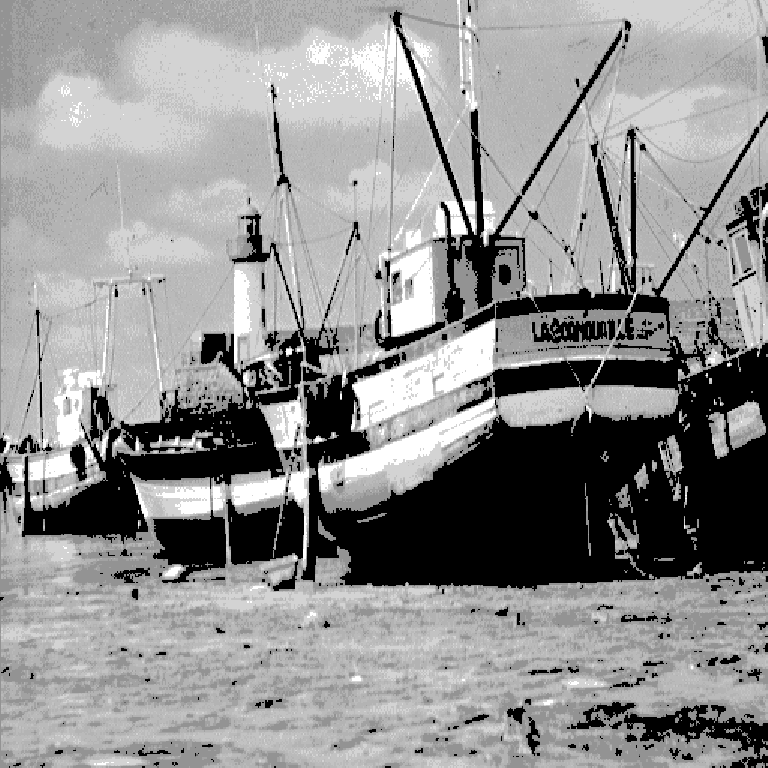
\includegraphics[width=0.13\columnwidth]{../test_results/boat_6_mode_img.pdf}}&
            \adjustbox{valign=c}{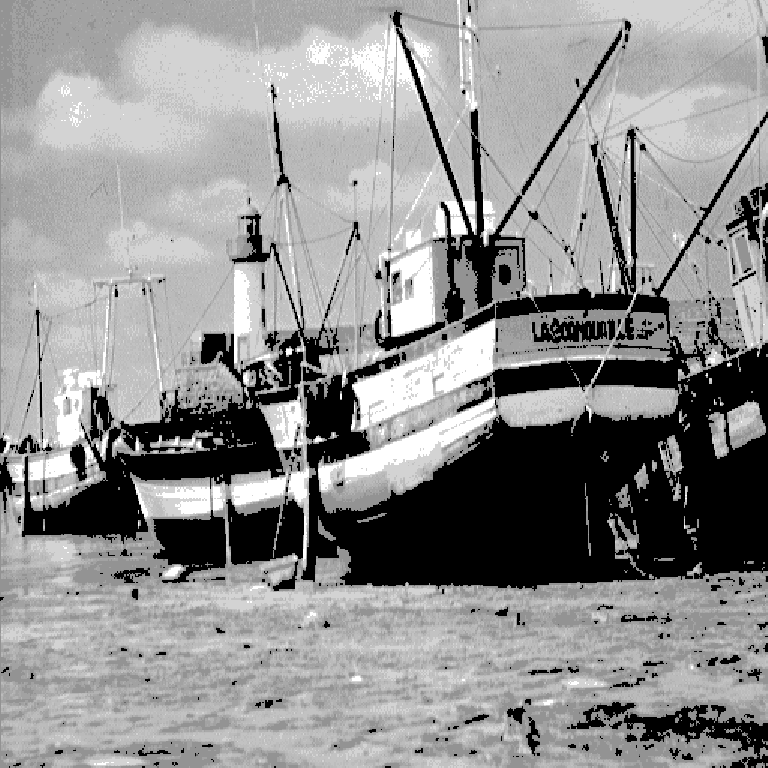
\includegraphics[width=0.13\columnwidth]{../test_results/boat_8_mode_img.pdf}}&
            \adjustbox{valign=c}{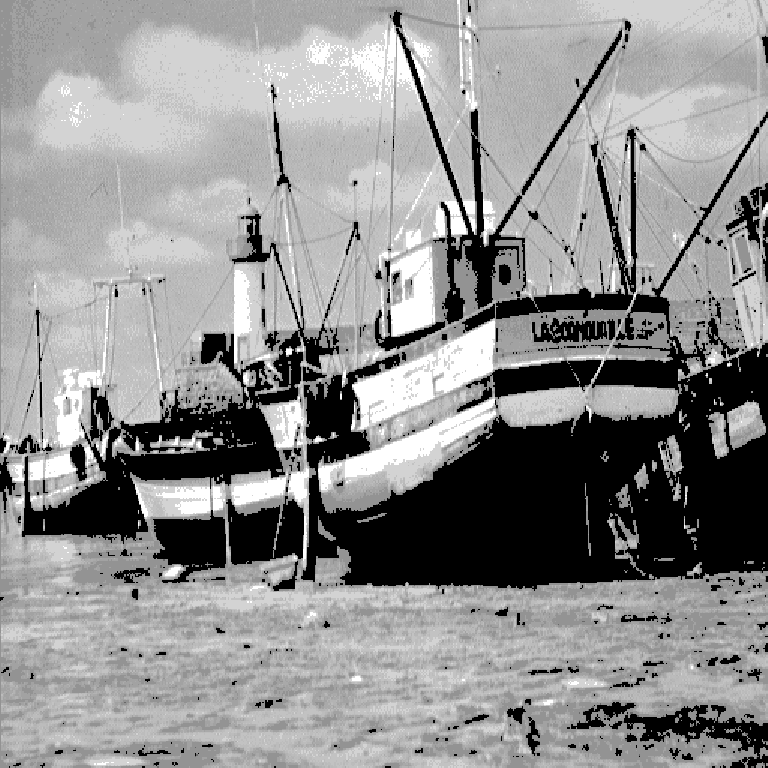
\includegraphics[width=0.13\columnwidth]{../test_results/boat_10_mode_img.pdf}}\\
    \end{tabular}
    \bigskip
                
        
    \fontsize{32}{32}\selectfont % Sets font size to 14pt with 16pt line spacing
    \vspace*{12mm}
    \centerline{\textbf{house}}
    \vspace*{12mm}
    \normalsize % Resets to the base font size
    \def\arraystretch{0.2} % Adjust row spacing if needed
    \fontsize{12}{12}

    \begin{tabular}{ @{}c@{\hspace{0pt}}ccccccc }
        \multicolumn{1}{c}{} &
            \textbf{Thresholds} &
            \textbf{PSNR-vs-Level} &
            \textbf{Level 2} &
            \textbf{Level 4} &
            \textbf{Level 6} &
            \textbf{Level 8} &
            \textbf{Level 10} \\
        \vspace*{10mm}
        \adjustbox{valign=c}{\rotatebox[origin=c]{90}{\textbf{ house mean }}} &
            \adjustbox{valign=c}{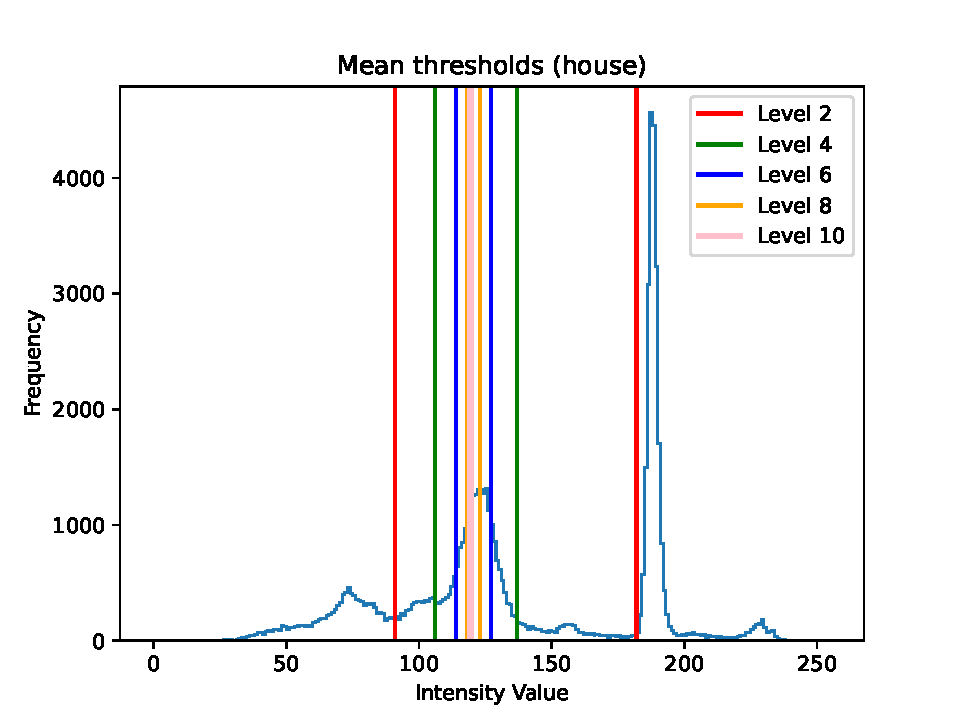
\includegraphics[width=0.13\columnwidth]{../test_results/house_mean.pdf}}&
            \adjustbox{valign=c}{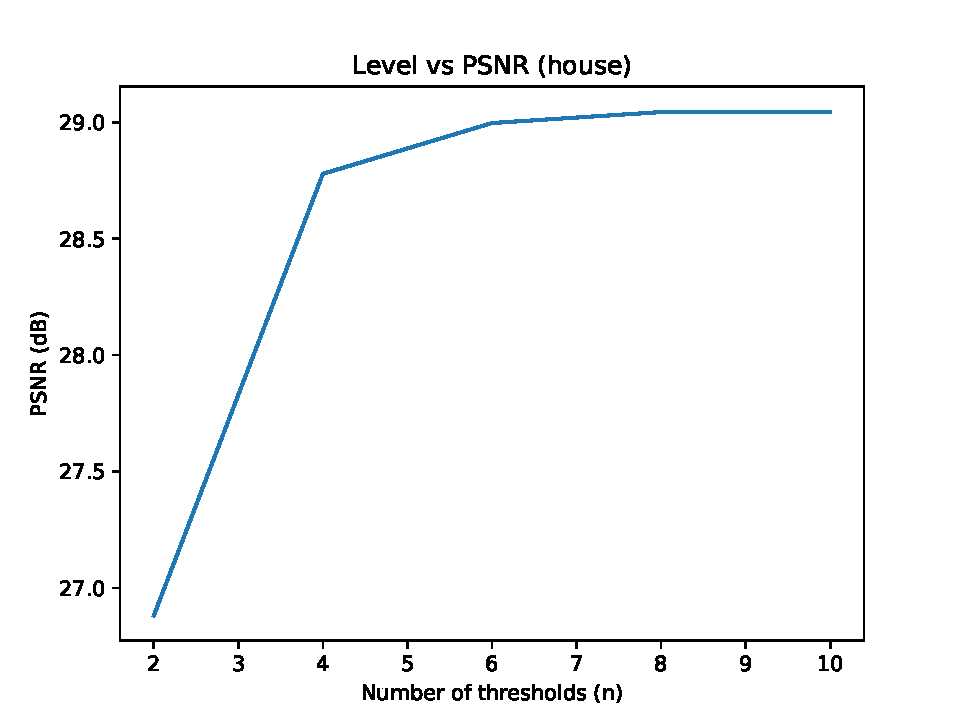
\includegraphics[width=0.13\columnwidth]{../test_results/house_mean_psnr.pdf}}&
            \adjustbox{valign=c}{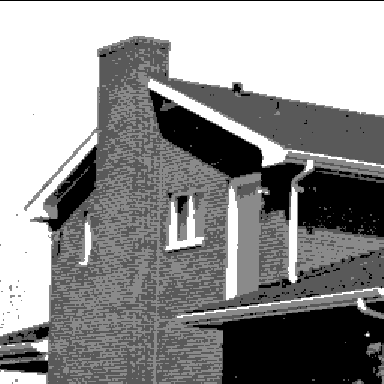
\includegraphics[width=0.13\columnwidth]{../test_results/house_2_mean_img.pdf}}&
            \adjustbox{valign=c}{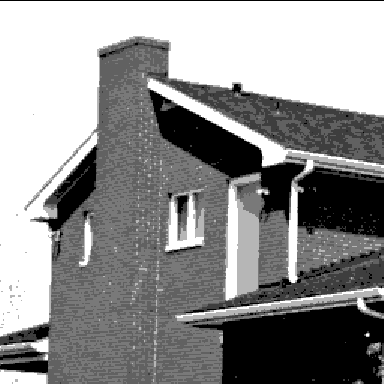
\includegraphics[width=0.13\columnwidth]{../test_results/house_4_mean_img.pdf}}&
            \adjustbox{valign=c}{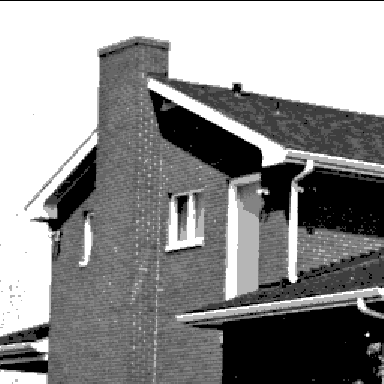
\includegraphics[width=0.13\columnwidth]{../test_results/house_6_mean_img.pdf}}&
            \adjustbox{valign=c}{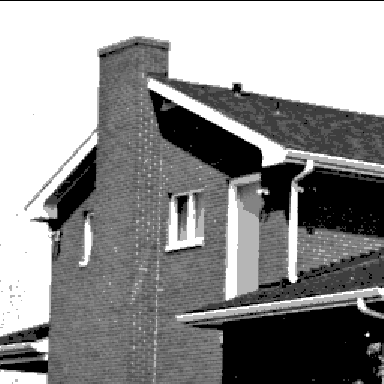
\includegraphics[width=0.13\columnwidth]{../test_results/house_8_mean_img.pdf}}&
            \adjustbox{valign=c}{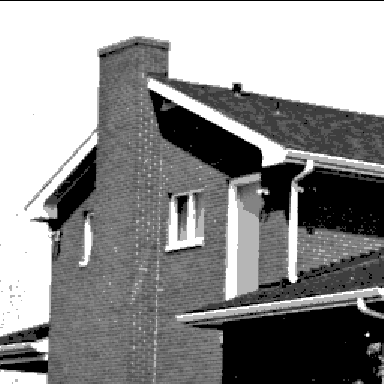
\includegraphics[width=0.13\columnwidth]{../test_results/house_10_mean_img.pdf}}\\
        \vspace*{6mm}
        \adjustbox{valign=c}{\rotatebox[origin=c]{90}{\textbf{ house mode }}} &
            \adjustbox{valign=c}{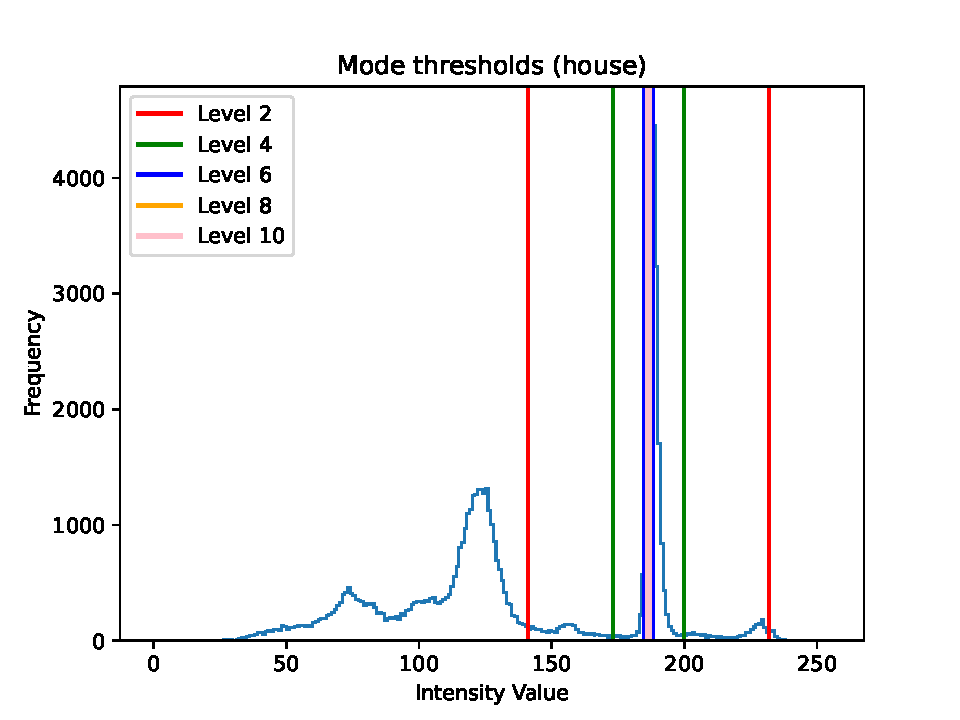
\includegraphics[width=0.13\columnwidth]{../test_results/house_mode.pdf}}&
            \adjustbox{valign=c}{\includegraphics[width=0.13\columnwidth]{../test_results/house_mode_psnr.pdf}}&
            \adjustbox{valign=c}{\includegraphics[width=0.13\columnwidth]{../test_results/house_2_mode_img.pdf}}&
            \adjustbox{valign=c}{\includegraphics[width=0.13\columnwidth]{../test_results/house_4_mode_img.pdf}}&
            \adjustbox{valign=c}{\includegraphics[width=0.13\columnwidth]{../test_results/house_6_mode_img.pdf}}&
            \adjustbox{valign=c}{\includegraphics[width=0.13\columnwidth]{../test_results/house_8_mode_img.pdf}}&
            \adjustbox{valign=c}{\includegraphics[width=0.13\columnwidth]{../test_results/house_10_mode_img.pdf}}\\
    \end{tabular}
    \bigskip
                
        
    \fontsize{32}{32}\selectfont % Sets font size to 14pt with 16pt line spacing
    \vspace*{12mm}
    \centerline{\textbf{jet}}
    \vspace*{12mm}
    \normalsize % Resets to the base font size
    \def\arraystretch{0.2} % Adjust row spacing if needed
    \fontsize{12}{12}

    \begin{tabular}{ @{}c@{\hspace{0pt}}ccccccc }
        \multicolumn{1}{c}{} &
            \textbf{Thresholds} &
            \textbf{PSNR-vs-Level} &
            \textbf{Level 2} &
            \textbf{Level 4} &
            \textbf{Level 6} &
            \textbf{Level 8} &
            \textbf{Level 10} \\
        \vspace*{10mm}
        \adjustbox{valign=c}{\rotatebox[origin=c]{90}{\textbf{ jet mean }}} &
            \adjustbox{valign=c}{\includegraphics[width=0.13\columnwidth]{../test_results/jet_mean.pdf}}&
            \adjustbox{valign=c}{\includegraphics[width=0.13\columnwidth]{../test_results/jet_mean_psnr.pdf}}&
            \adjustbox{valign=c}{\includegraphics[width=0.13\columnwidth]{../test_results/jet_2_mean_img.pdf}}&
            \adjustbox{valign=c}{\includegraphics[width=0.13\columnwidth]{../test_results/jet_4_mean_img.pdf}}&
            \adjustbox{valign=c}{\includegraphics[width=0.13\columnwidth]{../test_results/jet_6_mean_img.pdf}}&
            \adjustbox{valign=c}{\includegraphics[width=0.13\columnwidth]{../test_results/jet_8_mean_img.pdf}}&
            \adjustbox{valign=c}{\includegraphics[width=0.13\columnwidth]{../test_results/jet_10_mean_img.pdf}}\\
        \vspace*{6mm}
        \adjustbox{valign=c}{\rotatebox[origin=c]{90}{\textbf{ jet mode }}} &
            \adjustbox{valign=c}{\includegraphics[width=0.13\columnwidth]{../test_results/jet_mode.pdf}}&
            \adjustbox{valign=c}{\includegraphics[width=0.13\columnwidth]{../test_results/jet_mode_psnr.pdf}}&
            \adjustbox{valign=c}{\includegraphics[width=0.13\columnwidth]{../test_results/jet_2_mode_img.pdf}}&
            \adjustbox{valign=c}{\includegraphics[width=0.13\columnwidth]{../test_results/jet_4_mode_img.pdf}}&
            \adjustbox{valign=c}{\includegraphics[width=0.13\columnwidth]{../test_results/jet_6_mode_img.pdf}}&
            \adjustbox{valign=c}{\includegraphics[width=0.13\columnwidth]{../test_results/jet_8_mode_img.pdf}}&
            \adjustbox{valign=c}{\includegraphics[width=0.13\columnwidth]{../test_results/jet_10_mode_img.pdf}}\\
    \end{tabular}
    \bigskip
                
        
    \fontsize{32}{32}\selectfont % Sets font size to 14pt with 16pt line spacing
    \vspace*{12mm}
    \centerline{\textbf{lena}}
    \vspace*{12mm}
    \normalsize % Resets to the base font size
    \def\arraystretch{0.2} % Adjust row spacing if needed
    \fontsize{12}{12}

    \begin{tabular}{ @{}c@{\hspace{0pt}}ccccccc }
        \multicolumn{1}{c}{} &
            \textbf{Thresholds} &
            \textbf{PSNR-vs-Level} &
            \textbf{Level 2} &
            \textbf{Level 4} &
            \textbf{Level 6} &
            \textbf{Level 8} &
            \textbf{Level 10} \\
        \vspace*{10mm}
        \adjustbox{valign=c}{\rotatebox[origin=c]{90}{\textbf{ lena mean }}} &
            \adjustbox{valign=c}{\includegraphics[width=0.13\columnwidth]{../test_results/lena_mean.pdf}}&
            \adjustbox{valign=c}{\includegraphics[width=0.13\columnwidth]{../test_results/lena_mean_psnr.pdf}}&
            \adjustbox{valign=c}{\includegraphics[width=0.13\columnwidth]{../test_results/lena_2_mean_img.pdf}}&
            \adjustbox{valign=c}{\includegraphics[width=0.13\columnwidth]{../test_results/lena_4_mean_img.pdf}}&
            \adjustbox{valign=c}{\includegraphics[width=0.13\columnwidth]{../test_results/lena_6_mean_img.pdf}}&
            \adjustbox{valign=c}{\includegraphics[width=0.13\columnwidth]{../test_results/lena_8_mean_img.pdf}}&
            \adjustbox{valign=c}{\includegraphics[width=0.13\columnwidth]{../test_results/lena_10_mean_img.pdf}}\\
        \vspace*{6mm}
        \adjustbox{valign=c}{\rotatebox[origin=c]{90}{\textbf{ lena mode }}} &
            \adjustbox{valign=c}{\includegraphics[width=0.13\columnwidth]{../test_results/lena_mode.pdf}}&
            \adjustbox{valign=c}{\includegraphics[width=0.13\columnwidth]{../test_results/lena_mode_psnr.pdf}}&
            \adjustbox{valign=c}{\includegraphics[width=0.13\columnwidth]{../test_results/lena_2_mode_img.pdf}}&
            \adjustbox{valign=c}{\includegraphics[width=0.13\columnwidth]{../test_results/lena_4_mode_img.pdf}}&
            \adjustbox{valign=c}{\includegraphics[width=0.13\columnwidth]{../test_results/lena_6_mode_img.pdf}}&
            \adjustbox{valign=c}{\includegraphics[width=0.13\columnwidth]{../test_results/lena_8_mode_img.pdf}}&
            \adjustbox{valign=c}{\includegraphics[width=0.13\columnwidth]{../test_results/lena_10_mode_img.pdf}}\\
    \end{tabular}
    \bigskip
                
        
    \fontsize{32}{32}\selectfont % Sets font size to 14pt with 16pt line spacing
    \vspace*{12mm}
    \centerline{\textbf{moon}}
    \vspace*{12mm}
    \normalsize % Resets to the base font size
    \def\arraystretch{0.2} % Adjust row spacing if needed
    \fontsize{12}{12}

    \begin{tabular}{ @{}c@{\hspace{0pt}}ccccccc }
        \multicolumn{1}{c}{} &
            \textbf{Thresholds} &
            \textbf{PSNR-vs-Level} &
            \textbf{Level 2} &
            \textbf{Level 4} &
            \textbf{Level 6} &
            \textbf{Level 8} &
            \textbf{Level 10} \\
        \vspace*{10mm}
        \adjustbox{valign=c}{\rotatebox[origin=c]{90}{\textbf{ moon mean }}} &
            \adjustbox{valign=c}{\includegraphics[width=0.13\columnwidth]{../test_results/moon_mean.pdf}}&
            \adjustbox{valign=c}{\includegraphics[width=0.13\columnwidth]{../test_results/moon_mean_psnr.pdf}}&
            \adjustbox{valign=c}{\includegraphics[width=0.13\columnwidth]{../test_results/moon_2_mean_img.pdf}}&
            \adjustbox{valign=c}{\includegraphics[width=0.13\columnwidth]{../test_results/moon_4_mean_img.pdf}}&
            \adjustbox{valign=c}{\includegraphics[width=0.13\columnwidth]{../test_results/moon_6_mean_img.pdf}}&
            \adjustbox{valign=c}{\includegraphics[width=0.13\columnwidth]{../test_results/moon_8_mean_img.pdf}}&
            \adjustbox{valign=c}{\includegraphics[width=0.13\columnwidth]{../test_results/moon_10_mean_img.pdf}}\\
        \vspace*{6mm}
        \adjustbox{valign=c}{\rotatebox[origin=c]{90}{\textbf{ moon mode }}} &
            \adjustbox{valign=c}{\includegraphics[width=0.13\columnwidth]{../test_results/moon_mode.pdf}}&
            \adjustbox{valign=c}{\includegraphics[width=0.13\columnwidth]{../test_results/moon_mode_psnr.pdf}}&
            \adjustbox{valign=c}{\includegraphics[width=0.13\columnwidth]{../test_results/moon_2_mode_img.pdf}}&
            \adjustbox{valign=c}{\includegraphics[width=0.13\columnwidth]{../test_results/moon_4_mode_img.pdf}}&
            \adjustbox{valign=c}{\includegraphics[width=0.13\columnwidth]{../test_results/moon_6_mode_img.pdf}}&
            \adjustbox{valign=c}{\includegraphics[width=0.13\columnwidth]{../test_results/moon_8_mode_img.pdf}}&
            \adjustbox{valign=c}{\includegraphics[width=0.13\columnwidth]{../test_results/moon_10_mode_img.pdf}}\\
    \end{tabular}
    \bigskip
                
        
    \fontsize{32}{32}\selectfont % Sets font size to 14pt with 16pt line spacing
    \vspace*{12mm}
    \centerline{\textbf{peppers}}
    \vspace*{12mm}
    \normalsize % Resets to the base font size
    \def\arraystretch{0.2} % Adjust row spacing if needed
    \fontsize{12}{12}

    \begin{tabular}{ @{}c@{\hspace{0pt}}ccccccc }
        \multicolumn{1}{c}{} &
            \textbf{Thresholds} &
            \textbf{PSNR-vs-Level} &
            \textbf{Level 2} &
            \textbf{Level 4} &
            \textbf{Level 6} &
            \textbf{Level 8} &
            \textbf{Level 10} \\
        \vspace*{10mm}
        \adjustbox{valign=c}{\rotatebox[origin=c]{90}{\textbf{ peppers mean }}} &
            \adjustbox{valign=c}{\includegraphics[width=0.13\columnwidth]{../test_results/peppers_mean.pdf}}&
            \adjustbox{valign=c}{\includegraphics[width=0.13\columnwidth]{../test_results/peppers_mean_psnr.pdf}}&
            \adjustbox{valign=c}{\includegraphics[width=0.13\columnwidth]{../test_results/peppers_2_mean_img.pdf}}&
            \adjustbox{valign=c}{\includegraphics[width=0.13\columnwidth]{../test_results/peppers_4_mean_img.pdf}}&
            \adjustbox{valign=c}{\includegraphics[width=0.13\columnwidth]{../test_results/peppers_6_mean_img.pdf}}&
            \adjustbox{valign=c}{\includegraphics[width=0.13\columnwidth]{../test_results/peppers_8_mean_img.pdf}}&
            \adjustbox{valign=c}{\includegraphics[width=0.13\columnwidth]{../test_results/peppers_10_mean_img.pdf}}\\
        \vspace*{6mm}
        \adjustbox{valign=c}{\rotatebox[origin=c]{90}{\textbf{ peppers mode }}} &
            \adjustbox{valign=c}{\includegraphics[width=0.13\columnwidth]{../test_results/peppers_mode.pdf}}&
            \adjustbox{valign=c}{\includegraphics[width=0.13\columnwidth]{../test_results/peppers_mode_psnr.pdf}}&
            \adjustbox{valign=c}{\includegraphics[width=0.13\columnwidth]{../test_results/peppers_2_mode_img.pdf}}&
            \adjustbox{valign=c}{\includegraphics[width=0.13\columnwidth]{../test_results/peppers_4_mode_img.pdf}}&
            \adjustbox{valign=c}{\includegraphics[width=0.13\columnwidth]{../test_results/peppers_6_mode_img.pdf}}&
            \adjustbox{valign=c}{\includegraphics[width=0.13\columnwidth]{../test_results/peppers_8_mode_img.pdf}}&
            \adjustbox{valign=c}{\includegraphics[width=0.13\columnwidth]{../test_results/peppers_10_mode_img.pdf}}\\
    \end{tabular}
    \bigskip
                
        \end{document}